% !TEX root = ../../prj4projektdokumentation.tex

\subsection{Total Harmonic Distortion}

Måleenheden indeholder en funktion til beregning af Total Harmonic Distortion (THD). THD er et udtryk for hvor stort indholdet af overharmoniske frekvenser er i et givent signal. Signalet som Måleneheden måler på, består ideelt set kun af grundfrekvensen på 50Hz. 

Udregningen af THD i Måleenheden udføres efter der er lavet Fourier analyse af signalet. Herefter udregnes THD ved at dele den kvadrede sum af alle overharmoniske amplituder med amplituden af den fundamentale frekvens. Den generelle formel for udregning af THD er vist i Ligning \ref{eq:THDgenerel}.
\begin{align}
	THD = \dfrac{\sqrt{\sum_{n=2}^{\infty}V_n^{2}}}{V_{1}}
	\label{eq:THDgenerel}
\end{align}
Måleenheder udregner THD på baggrund af de første 5 frekvensbins, inklusiv den fundamentale frekvens jf. ligning \ref{eq:THDME}.
\begin{align}
THD = \dfrac{\sqrt{V_2^{2}+V_3^{2}+V_4^{2}+V_5^{2}}}{V_{1}}
\label{eq:THDME}
\end{align}

\subsubsection{Test af THD beregning i Måleenhed}
\label{sek:THD}


Udregningen af THD i Måleenheden er testet ved at sammenligne med resultatet med en simulering i Matlab. I Matlab er der lavet et signal der svarer til et firkantsignal i frekvensdomænet, hvorefter der er udregnet THD for de første 5 frekvensbins. Matlab koden ses i Listing \ref{list:THDMatlab}. Resultatet af Matlabsimuleringen bliver

\begin{align}
	THD\_square\_theoretical = 0,3887
\end{align}



\lstset{caption={Beregning af THD for firkantsignal i Matlab},label={list:THDMatlab}
			language=Matlab,
			frame=single}
\begin{lstlisting}[language=Matlab] 
freq = 50;

%%% double check THD of square wave using the fourier series:
n = 1:10000;
freq_vec = freq*n;  % fourier series frequency vector
amp_vec = (4/pi)  * (1./n).*(mod(n,2)==1);

% compute THD by definition:
THD_square_theoretical = (sum(amp_vec(2:5).^2) / amp_vec(1)^2)^0.5
\end{lstlisting}


Herefter laves en test på Måleenheden. Forudsætning for testen er at sampling og Fourier-transformationen fungerer. Til testen bruges en funktionsgenerator til at lave det firkantsignal der skal måles på. Signalet forbindes til det analoge spændings input på PSOCen, hvorefter debuggeren i PSOC creator 4.0 startes. Værdien for THD i måleenheden bliver 
\begin{align}
THD_{måleenhed} = 0,391
\end{align}
hvilket er inden for de 10\% præcision specificeret i Ikke Funktionelle Krav (sektion \ref{subsec:ME}). På Figur \ref{fig:METHDtest} ses resultatet fra debuggeren og indstillingerne på funktionsgeneratoren. 

\begin{figure}[htbp] % (alternativt [H])
	\centering
	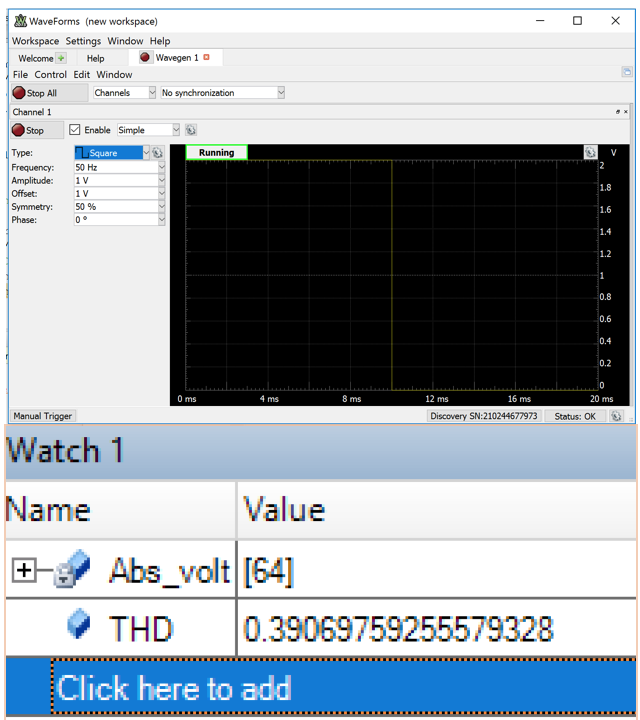
\includegraphics[width=0.6\textwidth]{Figure/METHDtest}
	\caption{Test af THD funktion på Måleenhed}
	\label{fig:METHDtest}
\end{figure}